\documentclass[a4paper, 11pt]{article}

\usepackage[utf8]{inputenc}
\usepackage{graphicx}
\usepackage[frenchb]{babel}
\usepackage{hyperref}
\usepackage{listings}
\usepackage{minted}
\usepackage{tcolorbox}
\usepackage{geometry}
\geometry{
 a4paper,
 left=15mm,
 right=15mm,
}

\begin{document}

\title{TP NoSQL\\Modélisation d'un système d'information de l'EMSE avec le moteur de base de données NoSQL Cassandra}
\author{Paul BREUGNOT, Nicolas LAGAILLARDIE}
\date{\today} 

\maketitle

\newpage

\tableofcontents

\newpage

\section{Création de la base de données}
\subsection{Oublier le modèle relationnel}

\paragraph{}
Nous avons initialement modélisé la base de données selon le diagramme de classe figure \ref{relationnal_diagram}\footnote{Construit grâce au logiciel OpenSource Modelio : \url{https://www.modelio.org/}}.

\begin{figure}[h]
\centering
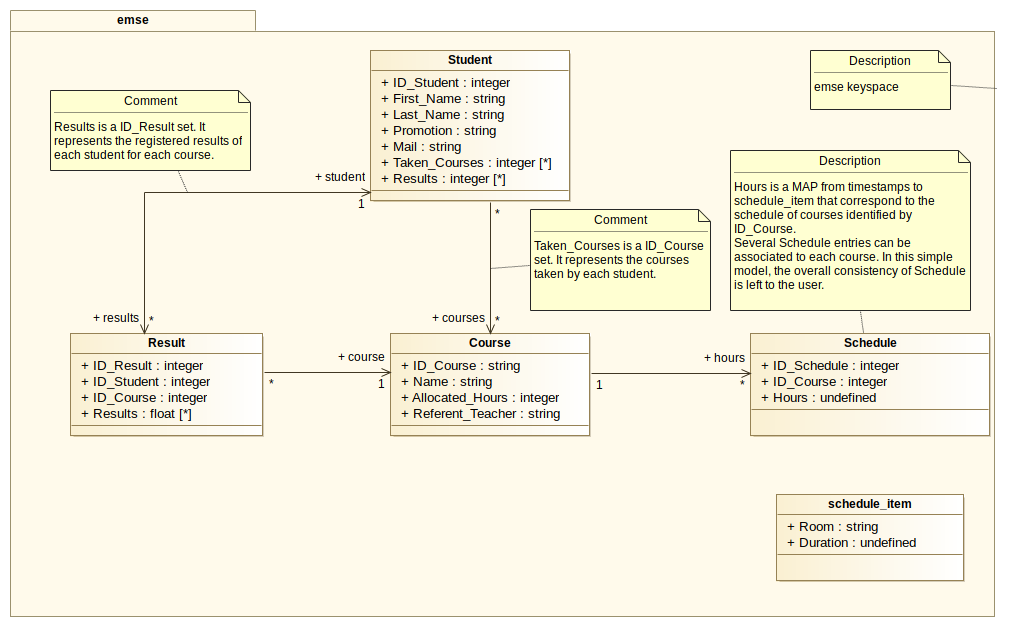
\includegraphics[width=\textwidth]{images/relationnal_class_diagram.png}
\caption{Modélisation \textbf{relationnelle} de la base de données.}
\label{relationnal_diagram}
\end{figure}

Bien qu'a priori cohérente, une telle implémentation n'est en réalité \textbf{pas utilisable} avec Cassandra et la langage CQL (même si toutes les tables peuvent être créées). En effet, ce modèle est clairement orienté sur les \textbf{relations} entre les tables permises par des \textbf{FOREIGN\_KEY}, une notion qui \textbf{n'existe pas dans un modèle orienté colonne}.

\paragraph{}
La première étape de création d'une base de données CQL est donc d'\emph{oublier} notre modèle relationnel couramment utilisé ainsi que les "bonnes pratiques" qui y sont associées. 

\subsection{Modélisation orientée colonnes}
\paragraph{}
En effet, dans une base de données relationnelle SQL, l'objectif est de réduire au maximum la duplication des données grâce à des relations et des tables de relations, tout en permettant la plus grande diversité de requêtes SQL possibles sur la table.

\paragraph{}
Le modèle de conception d'une base de données CQL est en réalité diamétralement opposé à ces pratiques. En effet, il est plutôt nécessaire d'anticiper certaines requêtes qui devront être faites sur la base de données, puis de construire autour de ces requêtes le modèle afin notamment de les optimiser.

\paragraph{}
Une fois les requêtes anticipées dans la limite du possible, le principe est de faire en sorte que chacune d'elle n'interroge \textbf{qu'une seule partition, soit une seule table} (le modèle relationnel est à partir d'ici totalement proscrit) afin d'obtenir des réponses dans un temps très bref.

\paragraph{}
Évidemment, il est toujours nécessaire d'effectuer plusieurs types de requêtes sur une même base de données. Ainsi en CQL, l'idée va être de \textbf{créer de nouvelles tables pour chaque type de requêtes}, possiblement avec une copie (non nécessairement synchronisée!) des données des autres tables, mais \textbf{organisées différemment} pour correspondre aux nouvelles requêtes de manière optimale.

\paragraph{}
La création de tables gigantesques et la duplication poussée à l'extrême des données dans une base CQL n'est ainsi pas un problème théorique d'une part, pratique d'autre part : en effet Cassandra est conçu pour opérer sur des cluster de machines. On suppose alors que l'espace de stockage n'est pas un problème, mais que l'objectif est réellement de réduire le temps d'accès aux données. Peu importe que les données auxquelles on accède soient répliquées 10 fois, potentiellement sur d'autres machines, l'élément important est que la copie des données auxquelles on souhaite accéder avec une certaine requête soit sur une unique partition.

\paragraph{}
Dans notre cas, nous allons supposer deux cas d'utilisation principaux de la base de données :
\begin{itemize}
\item On doit pouvoir, à partir d'un élève, accéder aux cours qu'il suit et à sont emploi du temps, et enfin accéder à ses résultats pour chaque cours.
\item On doit pouvoir, par cours, accéder à la liste des élèves qui suivent ce cours, éventuellement par promotion.
\end{itemize}
Il en résulte la structure de la base de données \textbf{orientée colonne} mise en place, avec deux tables principales, qui peut être représentée par le diagramme figure \ref{column_diagram}. 

\begin{figure}[h]
\centering
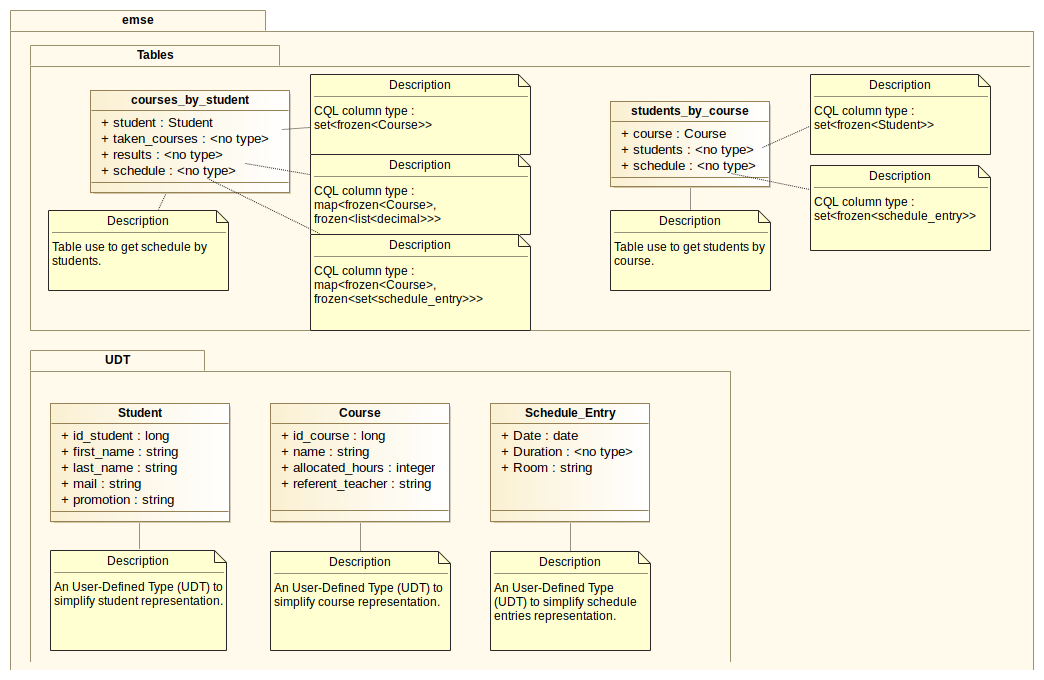
\includegraphics[width=\textwidth]{images/column_class_diagram.png}
\caption{Modélisation \textbf{orientée colonnes} de la base de données Cassandra utilisée.}
\label{column_diagram}
\end{figure}

\subsection{Script CQL}
Les sections suivantes exposent les requêtes CQL utilisées pour créer la base de données. Le script complet et exécutable avec \texttt{cqlsh} est disponible sur GitHub\footnote{\url{https://github.com/NicolasLagaillardie/Cassandra}}.

\subsubsection{Keyspace}

\begin{tcolorbox}
\begin{lstlisting}
CREATE KEYSPACE emse
WITH replication = {'class': 'SimpleStrategy', 'replication_factor': '1'}
\end{lstlisting}
\end{tcolorbox}

\subsubsection{User-Defined Types}
Les \emph{User-Defined Types}, ou \textbf{UDT} sont des structures de données pouvant être utilisées en CQL notamment pour simplifier la représentation des données, qui, on le rappelle, doivent dans l'idéal toute être contenues dans la même table pour un certain type de requêtes, ce qui mène rapidement à une structure de table très vaste et complexe.


\paragraph{UDT Student}
\subparagraph{}
Stocke les informations à propos des élèves. \texttt{promotion} vaut \texttt{"1A"}, \texttt{"2A"} ou \texttt{"3A"}.

\begin{tcolorbox}
\begin{lstlisting}
CREATE TYPE emse.student (
    id_student uuid,
    first_name text,
    last_name text,
    mail text,
    promotion text
);
\end{lstlisting}
\end{tcolorbox}

\paragraph{UDT Course}
\subparagraph{}
Type représentant les cours disponibles.

\begin{tcolorbox}
\begin{lstlisting}
CREATE TYPE emse.course (
    id_course uuid,
    name text,
    allocated_hours int,
    referent_teacher text
);

\end{lstlisting}
\end{tcolorbox}

\paragraph{UDT schedule\_entry}
\subparagraph{}
Un type permettant de simplifier la représentation d'un créneau de l'emploi du temps.

\begin{tcolorbox}
\begin{lstlisting}
CREATE TYPE emse.schedule_entry (
    date timestamp,
    duration duration,
    room text
);
\end{lstlisting}
\end{tcolorbox}

\subsubsection{Tables}

\paragraph{courses\_by\_student}

\subparagraph{}
On définie \texttt{student} en tant que \texttt{PRIMARY KEY}, car dans cette table les requêtes seront faite "par élève".
Ainsi, à chaque élève, on peut associer :
\begin{itemize}
\item Un ensemble de cours.
\item Un \texttt{map} des cours vers une \texttt{list} de \texttt{decimal} : la liste des notes de l'élève pour chaque cours.
\item Un \texttt{map} des cours vers un ensemble de créneaux horaires (\texttt{schedule\_entry}).
\end{itemize}
On notera que la cohérence de la liste de cours avec les résultats et créneaux associés n'est pas assurée autrement que par l'utilisateur.\\
On remarquera aussi ici la très grande réplication des données de l'emploi du temps pour chaque élève... mais pour chaque élève on aura un accès direct à son emploi du temps.

\small
\begin{tcolorbox}
\begin{lstlisting}
CREATE TABLE emse.courses_by_student (
    student frozen<student> PRIMARY KEY,
    results map<frozen<course>, frozen<list<decimal>>>,
    schedule map<frozen<course>, frozen<set<frozen<schedule_entry>>>>,
    taken_courses set<frozen<course>>
);
\end{lstlisting}
\end{tcolorbox}
\normalsize


\paragraph{students\_by\_course}
\subparagraph{}
Dans un modèle relationnel, ou avec l'aide d'une API plus haut niveau (par exemple, un script Python), on pourrait déduire le contenu de cette table à partir de la précédente, mais cela ne correspondrait pas au modèle de données CQL.

\subparagraph{}
On crée donc une nouvelle table, avec cette fois des éléments \texttt{course} pour \texttt{PRIMARY\_KEY}, auxquels on va associer un ensemble d'élèves et les créneaux de l'emploi du temps associés à chaque cours.

\begin{tcolorbox}
\begin{lstlisting}
CREATE TABLE emse.students_by_course (
    course frozen<course> PRIMARY KEY,
    schedule set<frozen<schedule_entry>>,
    students set<frozen<student>>
);
\end{lstlisting}
\end{tcolorbox}

\subsection{NoSQL}
\paragraph{}
Remarquons ici quelques spécificités du langage CQL.

\paragraph{Collections\\}
L'emploi de \texttt{collections} (\texttt{map}, \texttt{list}, \texttt{set}) est une différence notable par rapport au SQL. Leur utilisation est une fois de plus dans l'idée de représenter "proches" les données nécessitant un accès simultané.

\paragraph{\texttt{frozen}\\}
Le mot clé \texttt{frozen}, régulièrement utilisé notamment dans le cas de l'utilisation d'UDT, signifie qu'aucun champs de l'entité spécifiée ne pourra être modifié sans réécrire l'intégralité de l'entité. Le CQL impose l'utilisation de ce mot clé dans certaine situations (UDTs, collections au sein d'une collection...). Cela peut sembler contraignant et peut efficace, notamment dans le cas des emplois du temps :
\begin{lstlisting}
schedule map<frozen<course>, frozen<set<frozen<schedule_entry>>>>
\end{lstlisting}
Mais la "perte" de temps est en réalité peut significative, car même si on doit réécrire tout l'ensemble de créneaux d'un cours quand on change un créneau de ce cours, ce cas d'utilisation est en fait relativement rare car l'accès à la base de données se fait surtout en lecture, qui s'en trouve cette fois optimisée.

\section{Approvisionnement de la base de données avec Python}
La création de données test a été effectuée à l'aide d'un script Python. Les fonctions utilisées permettent de mettre en valeur les contraintes liées à l'ajout de données, qui on le rappelle sont essentiellement la responsabilité de l'utilisateur.\\
Le script complet est disponible sur GitHub\footnote{\url{https://github.com/NicolasLagaillardie/Cassandra}}.

\subsection{Implémentation des UDT}
De telles implémentations sont utiles pour grandement simplifier la génération des requêtes lors de l'appel de \texttt{session.execute()}, ainsi que pour régénérer les UDT depuis des requêtes \texttt{SELECT}.

\scriptsize
\begin{tcolorbox}
\begin{minted}[breaklines]{python}
class Student:

    def __init__(self, id_student, first_name, last_name, mail, promotion):
        self.id_student = id_student
        self.first_name = first_name
        self.last_name = last_name
        self.mail = mail
        self.promotion = promotion

    def __str__(self):
        # Automatically used when 'execute' is called to generate the CQL query.
        return "{id_student : " + str(self.id_student) +\
               ", first_name : '" + self.first_name +\
               "', last_name : '" + self.last_name +\
               "', mail : '" + self.mail +\
               "', promotion : '" + self.promotion +\
               "'}"

    @staticmethod
    def student_from_select(row_student):
        return Student(
            row_student.id_student,
            row_student.first_name,
            row_student.last_name,
            row_student.mail,
            row_student.promotion)


class Course:
    def __init__(self, id_course, name, allocated_hours, referent_teacher):
        self.id_course = id_course
        self.name = name
        self.allocated_hours = allocated_hours
        self.referent_teacher = referent_teacher

    def __str__(self):
        # Automatically used when 'execute' is called to generate the CQL query.
        return "{id_course : " + str(self.id_course) +\
               ", name : '" + self.name +\
               "', allocated_hours : " + str(self.allocated_hours) +\
               ", referent_teacher : '" + self.referent_teacher +\
               "'}"

    @staticmethod
    def course_from_select(row_course):
        return Course(
            row_course.id_course,
            row_course.name,
            row_course.allocated_hours,
            row_course.referent_teacher
        )


class Schedule_Entry:
    def __init__(self, date, duration, room):
        self.date = date
        self.duration = duration
        self.room = room

    def __str__(self):
        # Automatically used when 'execute' is called to generate the CQL query.
        return "{date : '" + str(self.date) + \
               "', duration : " + self.duration + \
               ", room : '" + self.room + \
               "'}"
\end{minted}
\end{tcolorbox}
\normalsize

\subsection{Initialisation}

Initialise un objet \texttt{session} grâce au package \texttt{cassandra-driver}.

\scriptsize

\begin{tcolorbox}
\begin{minted}[breaklines]{python}
# Cassandra driver
from cassandra.cluster import Cluster

def init_cassandra():
    cluster = Cluster()
    session = cluster.connect()

    # Select emse keyspace
    session.set_keyspace('emse')

    return session
\end{minted}
\end{tcolorbox}
\normalsize

\subsection{Course}
Pour créer des cours, il suffit de les ajouter à la table \texttt{students\_by\_course} sans spécifier de valeur pour les autres colonnes.

\scriptsize

\begin{tcolorbox}
\begin{minted}[breaklines]{python}
def add_courses(session):

    courses =\
        [Course(uuid1(), "Majeure Info", 159, "Jean"),
         Course(uuid1(), "Défi Big Data", 78, "Robert"),
         Course(uuid1(), "TB3 IA", 90, "Martin"),
         Course(uuid1(), "TB1 Traitement d_images", 40, "Paul")]

    print("Adding following entries to students_by_course : \n" + str(courses))

    # Add entries to table students_by_course
    for course in courses:
        session.execute(
            """
            INSERT INTO students_by_course (course)
            VALUES (%s)
            """,
            (course,)
            )
\end{minted}
\end{tcolorbox}
\normalsize

\subsection{Student}
Notons qu'on ajoute les élèves à la table \texttt{courses\_by\_student}, et qu'il est nécessaire de \textbf{manuellement} mettre à jours la table \texttt{students\_by\_course}, avec un "grand" nombre d'autres requêtes, pour la garder synchronisée. Ceci est très peu efficace, mais l'idée est qu'une telle opération est ponctuelle, et permet par la suite un accès rapide en lecture.

\scriptsize
\begin{tcolorbox}
\begin{minted}[breaklines]{python}
def add_students(session, entries_number=500):
    promotions = ("1A", "2A", "3A")

    # Add entries to table Student
    students = []

    courses = [Course.course_from_select(row.course)
               for row in session.execute("SELECT course FROM students_by_course")]

    for i in range(entries_number):

        ID_Student = uuid1()
        First_Name = "".join(choice(string.ascii_letters) for x in range(randint(5, 12)))
        Last_Name = "".join(choice(string.ascii_letters) for x in range(randint(5, 12)))
        Last_Name = Last_Name.upper()
        First_Name = First_Name.capitalize()
        Mail = First_Name.lower() + "." + First_Name.lower() + "@etu.emse.fr"
        Promotion = promotions[randint(0, 2)]

        Taken_Courses = []
        for course in courses:
            if randint(0, 1):
                Taken_Courses.append(course)

        students.append((Student(ID_Student, First_Name, Last_Name, Mail, Promotion), set(Taken_Courses)))

    print("Adding " + str(entries_number) + " random students to Student...")
    begin = datetime.now()

    print(students)
    for student in students:

        # Add entries to courses_by_student
        session.execute(
            """
            INSERT INTO courses_by_student (student, taken_courses)
            VALUES (%s, %s)
            """,
            student
        )

        # Update students_by_course
        for course in student[1]:
            session.execute(
                """
                UPDATE students_by_course SET students = students + {%s} WHERE course = %s
                """,
                (student[0], course)
            )

    end = datetime.now()
    print(str(entries_number) + " random students added in " + str((end - begin).total_seconds()) + " seconds.")
\end{minted}
\end{tcolorbox}
\normalsize

\subsection{Results}

Des notes aléatoires sont créées pour chaque matière de chaque élève. On a ici un premier exemple intéressant d'\texttt{UPDATE} d'une \texttt{map} en CQL.

\scriptsize
\begin{tcolorbox}
\begin{minted}[breaklines]{python}
def add_results(session, results_number_by_course=10):
    students = session.execute(
        """
        SELECT student, taken_courses FROM courses_by_student
        """)

    results = {}
    for row in students:
        student = Student.student_from_select(row.student)
        results[student] = {}
        if row.taken_courses is not None:
            for row_course in row.taken_courses:
                course = Course(
                    row_course.id_course,
                    row_course.name,
                    row_course.allocated_hours,
                    row_course.referent_teacher)
                marks = [randint(0, 20) for i in range(results_number_by_course)]
                results[student][course] = marks

    total_results = sum([len(results[student]) for student in results.keys()])
    print("Adding " + str(total_results) + " random hours to Schedule...")
    begin = datetime.now()
    for student in results.keys():
        for course in results[student].keys():
            session.execute(
                """
                UPDATE courses_by_student SET results[%s] = %s WHERE student = %s
                """,
                (course, results[student][course], student)
            )

    end = datetime.now()
    print(str(total_results) + " random results added in "
          + str((end - begin).total_seconds()) + " seconds.")
\end{minted}
\end{tcolorbox}

\normalsize
\subsection{Schedule}

Des entrées aléatoires mais réalistes sont générées. On constate bien ici l'importance de la gestion de la cohérence de la base de donnée au niveau utilisateur, et donc ici au niveau de la sur-couche Python :
\begin{itemize}
\item Les cours existant doivent être sélectionnés manuellement. Mais on pourrait insérer sans erreur des cours qui n'ont jamais été créés (c'est à dire ajoutés dans la table \texttt{students\_by\_course} comme précédemment).
\item La cohérence de l'emploi du temps n'est pas du tout assurée ici (des créneaux dans une même salle pourraient par exemple se chevaucher, des emplois du temps d'élèves pourraient être incompatibles...), mais si elle devait l'être il faudrait implémenter les tests et contraintes au niveau de cette sur-couche Python alors qu'on pourrait l'implémenter sous forme de contraintes dans une base de données SQL (cependant toujours au détriment des performances...). 
\end{itemize}
\scriptsize
\begin{tcolorbox}
\begin{minted}[breaklines]{python}
def add_schedule(session, entries_number_per_course=100):
    from datetime import datetime
    from random import randint

    blocks = ['D', 'A', 'E', 'F', 'G', 'H', 'J']

    schedule_entries = {}
    duration = "3h15m"  # A course duration as represented in CQL

    courses = [Course.course_from_select(row.course)
               for row in session.execute("SELECT course FROM students_by_course")]

    mid = int(entries_number_per_course / 2)

    for course in courses:
        schedule_entries[course] = []
        for j in range(mid):
            dt = datetime(2018, randint(1, 12), randint(1, 28), hour=8, minute=15)
            room = blocks[randint(0, 6)] + str(randint(0, 3)) + str(randint(0, 30))
            item = Schedule_Entry(dt, duration, room)
            schedule_entries[course].append(item)

        for j in range(mid, entries_number_per_course):
            dt = datetime(2018, randint(1, 12), randint(1, 28), hour=13, minute=30)
            room = blocks[randint(0, 6)] + str(randint(0, 3)) + str(randint(0, 30))
            item = Schedule_Entry(dt, duration, room)
            schedule_entries[course].append(item)

    total_hours = sum([len(schedule_entries[course]) for course in schedule_entries.keys()])
    print("Adding " + str(total_hours) + " random hours to Schedule...")
    begin = datetime.now()

    for course in schedule_entries.keys():

        schedule_entry_set = set(schedule_entries[course])

        # Add schedule to students_by_course
        session.execute(
            """
            UPDATE students_by_course SET schedule = %s WHERE course = %s
            """,
            (schedule_entry_set, course)
        )

        # Update courses_by_students
        for student in [Student.student_from_select(row.student)
                        for row in session.execute("SELECT student FROM courses_by_student")]:

            schedule_entry_str = "{"
            for schedule_entry in schedule_entry_set:
                schedule_entry_str += str(schedule_entry) + ", "
            schedule_entry_str = schedule_entry_str[0:-2] + "}"

            session.execute("UPDATE courses_by_student SET schedule[" + str(course) + "] = " + schedule_entry_str + " WHERE student = " + str(student))

    end = datetime.now()
    print(str(total_hours) + " random hours added in "
          + str((end - begin).total_seconds()) + " seconds.")
\end{minted}
\end{tcolorbox}
\normalsize

\section{Exemple de requêtes CQL}
\subsection{\texttt{students\_by\_course}}
\paragraph{}
Sélection du nom des cours disponibles :
\begin{tcolorbox}
\begin{lstlisting}
SELECT course.name FROM students_by_course;
\end{lstlisting}
\end{tcolorbox}

Résultats :
\begin{tcolorbox}
\begin{lstlisting}
 course.name
-------------------------

            Majeure Info
                  TB3 IA
 TB1 Traitement d_images
           Defi Big Data
\end{lstlisting}
\end{tcolorbox}

\paragraph{}
Sélection des élèves inscrit dans chaque cours :
\begin{tcolorbox}
\begin{lstlisting}
SELECT course, students FROM students_by_course;
\end{lstlisting}
\end{tcolorbox}
Si on veut accéder seulement aux nombre d'inscrits dans chaque cours, il est nécessaire de faire la même requête puis de calculer la taille de \texttt{students} avec une fonction Cassandra, un script Python...

\paragraph{}
Sélection de l'ensemble des créneaux horaires associés à chaque cours :
\begin{tcolorbox}
\begin{lstlisting}
SELECT course, schedule FROM students_by_course;
\end{lstlisting}
\end{tcolorbox}

\subsection{\texttt{courses\_by\_students}}

\paragraph{}
Sélection des prénoms, noms et adresse mail des élèves :
\scriptsize
\begin{tcolorbox}
\begin{lstlisting}
SELECT student.first_name, student.last_name, student.mail FROM courses_by_student;
\end{lstlisting}
\end{tcolorbox}
\normalsize
Notons que les clauses \texttt{WHERE} ne peuvent s'appliquer aux champs d'un UDT (par exemple : \texttt{student.promotion})...

\paragraph{}
Sélection des cours suivis par chaque élèves :
\begin{tcolorbox}
\begin{lstlisting}
SELECT student, taken_courses FROM courses_by_student;
\end{lstlisting}
\end{tcolorbox}

\paragraph{}
Sélection des cours suivis par chaque élève :
\begin{tcolorbox}
\begin{lstlisting}
SELECT student, taken_courses FROM courses_by_student;
\end{lstlisting}
\end{tcolorbox}

\paragraph{}
Sélection des résultats de chaque élève :
\begin{tcolorbox}
\begin{lstlisting}
SELECT student, results FROM courses_by_student;
\end{lstlisting}
\end{tcolorbox}

\paragraph{}
Sélection de l'emploi du temps de chaque élève :
\begin{tcolorbox}
\begin{lstlisting}
SELECT student, schedule FROM courses_by_student;
\end{lstlisting}
\end{tcolorbox}


\section{Conclusion}
\paragraph{}
L'implémentation d'une base de données Cassandra nous a permis d'explorer les possibilités d'un base de données non relationnelle.

\paragraph{}
Bien qu'efficaces en terme de temps d'exécution et optimisées pour certains cas d'utilisation très précis, les requêtes CQL sont cependant très peu flexibles et limitées. La création du modèle peut s'avérer contre intuitive et requérir un espace de stockage indisponible dans le cas de bases de données conséquentes, en raison de la duplication des données. La synchronisation des données entre les tables peut également poser problème.
\end{document}